\documentclass[11pt,class=report,crop=false]{standalone}
\usepackage[screen]{../python}



\begin{document}


%====================================================================
\chapitre{Utiliser un ordinateur quantique (avec Qiskit)}
%====================================================================

\insertvideo{yGzmA98D0eU}{partie 2.1. Un premier circuit quantique}

\insertvideo{7tO15IFNtMQ}{partie 2.2 Un qubit}

\insertvideo{SL4nMgMwPbI}{partie 2.3 Deux qubits}

\insertvideo{etra0QQUUOg}{partie 2.4 Utiliser un vrai ordinateur quantique}


\objectifs{Le but est de programmer des circuits quantiques et de simuler les résultats. Mais nous allons aussi utiliser un véritable ordinateur quantique.}

\index{qiskit}
\index{circuit quantique}

%%%%%%%%%%%%%%%%%%%%%%%%%%%%%%%%%%%%%%%%%%%%%%%%%%%%%%%%%%%%%%%%%%%%%
\section{Un premier circuit quantique}

On se jette  l'eau et on réalise notre premier circuit quantique.
Nous utilisons le langage de programmation \Python{} et la librairie \qiskit{}
fournie par IBM.

%--------------------------------------------------------------------
\subsection{Le circuit}

Il s'agit de programmer le circuit suivant.
$$
\Qcircuit @C=1em @R=1em {
\lstick{\ket0} & \gate{H} & \meter & \qwa \\
}
$$


On part donc de l'état initial $\ket0$, on applique une porte de Hadamard, l'état quantique devient donc $\frac1{\sqrt2}\ket0 + \frac1{\sqrt2}\ket1$. On termine par une mesure qui renvoie un bit classique $0$ ou $1$ avec ici chacun la probabilité $1/2$.

Pour mieux représenter la réalité de ce circuit, on l'écrit sur deux lignes. La première ligne correspond au qubit, noté $q$ et à sa transformation, la seconde ligne correspond au bit classique, noté $c$, qui sert à stocker la mesure du qubit.

$$
\Qcircuit @C=1em @R=1em {
\lstick{q=\ket0} & \gate{H} & \meter   & \qw \\
\lstick{c=0}     & \qw      & \qw \qwx &   \qwa 
}
$$

\bigskip

\emph{Remarque importante.} Noter la différence avec les circuits rencontrés dans le premier chapitre :  les circuits sont ici initialisés avec un état initial,  $\ket0$ pour les qubits et $0$ pour les bits classiques.


%--------------------------------------------------------------------
\subsection{Le programme}

\begin{lstlisting}
import qiskit as q

### Partie A. Préparation

# On simule un ordinateur quantique
simulator = q.Aer.get_backend('qasm_simulator')

### Partie B. Construction du circuit

# Circuit quantique avec un qubit et une mesure
circuit = q.QuantumCircuit(1, 1)

# Une porte de Hadamard
circuit.h(0)

# Mesure du qubit (donne un bit classique)
circuit.measure(0, 0)

# Affichage du circuit
print(circuit.draw(output='text'))  

### Partie C. Exécution 

# Lancer de 1000 simulations
job = q.execute(circuit, simulator, shots=1000)

### Partie D. Résultats et visualisation

result = job.result()

# Comptage
counts = result.get_counts(circuit)
print("Nombre de '0' et de '1':",counts)

# Diagramme en barres
import matplotlib.pyplot as plt
q.visualization.plot_histogram(counts)
plt.show()
\end{lstlisting}

%--------------------------------------------------------------------
\subsection{Explications et résultats}

On reprend pas à pas le programme ci-dessus avec des explications et les résultats.

\textbf{Partie A. Préparation}

\begin{itemize}
  \item Le module \Python{} à importer au préalable est le module \qiskit{}, on abrège son nom par la seule lettre \ci{q}.
  \item Pour l'instant on n'utilise pas un véritable ordinateur quantique, mais on transforme notre machine en un simulateur avec l'option \ci{'qasm_simulator'}.
\end{itemize}

\bigskip
\textbf{Partie B. Construction du circuit}

On commence par déclarer l'architecture du circuit :
\mycenterline{\ci{circuit = q.QuantumCircuit(1, 1)}}
L'instruction définit un circuit quantique, nommé \ci{circuit}, et déclare le nombre de bits quantiques (ici $1$) suivi du nombre de bits classiques (ici $1$ également, pour la mesure).

On construit ensuite le circuit de la gauche vers la droite :
\begin{itemize}
  \item on ajoute une porte \mygate{H} de Hadamard pour le qubit numéro $0$ : \ci{circuit.h(0)}.
  \item on mesure le qubit numéro $0$ et on envoie le résultat sur le bit classique numéro $0$ : \ci{circuit.measure(0, 0)}.
\end{itemize}

Le programme affiche ensuite une version texte de notre circuit, ce qui permet de vérifier que tout est bien en place. 
\begin{center}
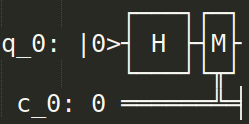
\includegraphics[scale=\myscale,scale=0.5]{figures/fig-circuit-texte}
\end{center}
Comme l'entrée n'a pas été précisée, c'est, comme mentionné sur l'affichage ci-dessus, la valeur par défaut qui sera utilisée, à savoir $\ket0$.

\bigskip
\textbf{Partie C. \'Exécution}

Le travail de simulation commence. 
Un test du circuit conduit à une mesure, avec une sortie $0$ ou $1$  (la valeur exacte du qubit dans le circuit n'est pas accessible). Une seule valeur ne permet pas de conclure sur la nature du circuit, c'est pourquoi on effectue une simulation avec un grand nombre de lancers (\emph{shots}). 
\mycenterline{\ci{job = q.execute(circuit, simulator, shots=1000)}}





\bigskip
\textbf{Partie D. Résultats et visualisation}

Voici un exemple de résultat renvoyé.
\mycenterline{
\ci{Nombre de '0' et de '1': {'0': 519, '1': 481}}
}
Bien sûr, chaque simulation a une part d'aléatoire et conduit à des résultats différents.
Cependant, selon la loi des grands nombres, par exemple avec $1000$ lancers, la proportion de $0$ et de $1$ obtenue doit se rapprocher de la probabilité attendue.
Ici les proportions de $0$ et de $1$ sont effectivement proches de la probabilité $\frac12$ attendue :
$$p_0 = \frac{519}{1000}=0.519 \qquad \text{ et } \qquad p_1 = \frac{481}{1000} = 0.481.$$

On dispose aussi d'un affichage graphique.
\begin{center}
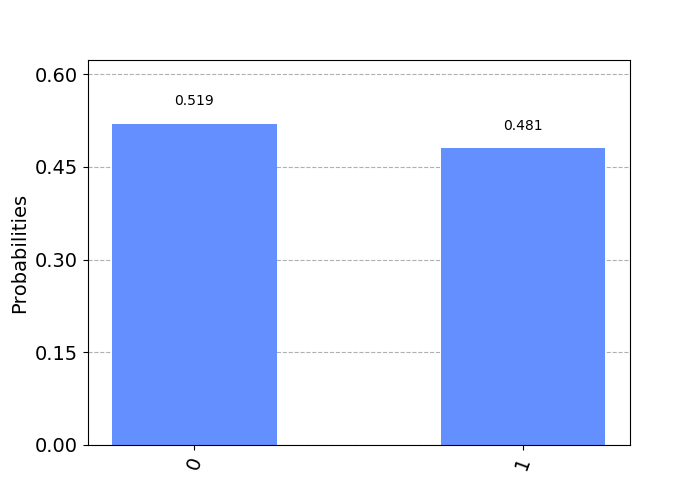
\includegraphics[scale=\myscale,scale=0.5]{figures/fig-qiskit-01}
\end{center}

En conclusion, notre circuit, qui réalise la mesure du qubit $\frac1{\sqrt2}\ket0 + \frac1{\sqrt2}\ket1$, fonctionne bien comme attendu et renvoie $0$ ou $1$ avec chacun une probabilité $\frac12$.


%%%%%%%%%%%%%%%%%%%%%%%%%%%%%%%%%%%%%%%%%%%%%%%%%%%%%%%%%%%%%%%%%%%%%
\section{Un qubit}

\index{qubit!qiskit}

%--------------------------------------------------------------------
\subsection{Nombres complexes avec \Python}

Le nombre complexe $z =\frac{\sqrt3}{2} + \frac12\ii$ s'affiche avec \Python{} de la manière suivante :
\mycenterline{\ci{0.8660254037844386-0.5j}}

Le nombre $\ii$ est représenté par \ci{j} (ou plus exactement par \ci{1j}). Malheureusement \Python{} ne fait pas de calculs exacts, il utilise des nombres flottants pour la partie réelle et pour la partie imaginaire.

Voici comment définir et afficher ce nombre complexe :
\begin{lstlisting}
import numpy as np
z = np.sqrt(3)/2 + 1/2j
print(z)
print(abs(z))
print(1/z)
\end{lstlisting}
On manipule les nombres complexes comme les nombres réels : \ci{z1+z2},
\ci{z1*z2}, \ci{z**2}, \ci{1/z}.

Le module du nombre complexe $z$ est $1$, la valeur renvoyée par la fonction \ci{abs(z)} est \ci{0.99999...}



%--------------------------------------------------------------------
\subsection{Circuit}

Nous allons programmer un circuit encore plus simple que précédemment :
{\large$$
\Qcircuit @C=1em @R=1em {
 & \gate{X} &  \qwa \\
}
$$}

Deux différences majeures cependant :
\begin{itemize}
  \item Cette fois nous allons initialiser l'entrée par un qubit $\ket\psi$ quelconque (et non plus $\ket0$).
  \item Nous utiliserons un \og{}faux\fg{} ordinateur quantique afin d'obtenir les états quantiques. En effet un \og{}vrai\fg{} circuit quantique n'est pas pratique pour l'apprentissage car il ne permet d'obtenir que des probabilités approchées et pas les états quantiques de qubits.
\end{itemize}

%--------------------------------------------------------------------
\subsection{Le programme}
\label{ssec:progstate}

\begin{lstlisting}
### Partie A. Préparation

simulator = q.Aer.get_backend('statevector_simulator')

### Partie B. Construction du circuit

circuit = q.QuantumCircuit(1)

# Initialisation à la main : écriture algébrique
alpha0 = 3+1j
beta0 = 1-2j
norme = np.sqrt(abs(alpha0)**2 + abs(beta0)**2)
alpha, beta = alpha0/norme, beta0/norme
etat_initial = [alpha,beta]
qubit_initial = q.extensions.Initialize(etat_initial)
circuit.append(qubit_initial, [0])

# Circuit : une porte X
circuit.x(0)

# Partie C. Exécution 

job = q.execute(circuit, simulator)

# Partie D. Résultats

result = job.result()

coefficients = result.get_statevector()
print("Coefficient alpha:", coefficients[0])
print("Coefficient beta :", coefficients[1])
\end{lstlisting}

%--------------------------------------------------------------------
\subsection{Explications et résultats}

\begin{itemize}
  \item Cette fois le simulateur appelé est \ci{'statevector_simulator'}, ce qui nous permet de récupérer les états quantiques en plus de leur mesure. C'est pratique pour vérifier la validité de nos circuits mais cela ne correspond pas à la réalité physique !
  
  \item Cette fois, notre circuit est défini avec un seul qubit (indexé par $0$). La valeur par défaut de ce qubit est $\ket0$.
  
  \item Mais on va changer cette valeur, on souhaite comme qubit initial :
  $$\ket\psi  = (3+\ii) \ket0 + (1-2\ii)\ket1.$$
  Pour cela on définit $\alpha_0=3+\ii$, $\beta_0=1-2\ii$.
  
  Afin que l'entrée soit acceptée, il faut normaliser le qubit $\ket\psi$.
  On calcule donc la norme $\|\psi\| = \sqrt{|\alpha_0|^2+|\beta_0|^2}$. Et on définit
  $\alpha = \alpha_0/\|\psi\|$ et $\beta = \beta_0/\|\psi\|$. Ce qui nous permet de définir le qubit initial à l'aide de la commande \ci{Initialise([alpha,beta])}.
  
  \item On rajoute une porte de Pauli $X$ (qui échange les coefficients $\alpha$ et $\beta$ du qubit).
  
  \item On récupère les coefficients du qubit de sortie par la fonction \ci{get_statevector()}.
  
  \item Résultats. Notre qubit normalisé en entrée est :
  $$\ket{\psi'} = (0.7746+0.2582\ii)\ket0 + (0.2582-0.5164\ii)\ket1$$
  La sortie obtenue :
  $$(0.2582-0.5164\ii)\ket0 + (0.7746+0.2582\ii)\ket1$$
  est bien $X(\ket{\psi'})$.
\end{itemize}


Toutes les portes classiques sont disponibles : la porte \mygate{H} de Hadamard, les portes de Pauli \mygate{X}, \mygate{Y}, \mygate{Z}\ldots

\begin{exercicecours}
On considère le circuit : 
$$
\Qcircuit @C=1em @R=1em {
 & \gate{H} & \gate{X} & \gate{Y} & \qwa \\
}
$$
et le qubit d'entrée
$$\ket\psi = \frac{\sqrt3}{2} \ket 0 + \frac{1-\ii}{2\sqrt2}\ket1$$
qui est un qubit de norme $1$.
Calculer la sortie à l'aide de la machine et vérifier vos calculs à la main.
\end{exercicecours}



%%%%%%%%%%%%%%%%%%%%%%%%%%%%%%%%%%%%%%%%%%%%%%%%%%%%%%%%%%%%%%%%%%%%%
\section{Deux qubits}

\index{qubit!qiskit}

%--------------------------------------------------------------------
\subsection{Le circuit}

$$
\Qcircuit @C=1em @R=1em {
\lstick{\ket0} & \gate{H} & \ctrl{1} & \qw & \meter & \qw & \qwa \\
\lstick{\ket0} & \gate{X} & \targ  &\gate{H}   & \meter & \qwa \\
}
$$
\medskip

Voici une représentation plus réaliste de ce circuit, avec les deux lignes pour les bits classiques qui servent de stockage pour les mesures :
$$
\Qcircuit @C=1em @R=1em {
\lstick{q_0=\ket0} & \gate{H} & \ctrl{1} & \qw  & \meter     & \qw    & \qw \\
\lstick{q_1=\ket0} & \gate{X} & \targ    & \gate{H}  &\qw    & \meter & \qw \\
\lstick{c_0=0}     & \qw      & \qw   &\qw   & \qw \qwx[-2] & \qw    & \qwa \\ 
\lstick{c_1=0}     & \qw      & \qw      & \qw      & \qw   & \qw \qwx[-2] & \qwa \\
}
$$

%--------------------------------------------------------------------
\subsection{Le programme}

\begin{lstlisting}
### Partie A. Préparation
simulator = q.Aer.get_backend('qasm_simulator')

### Partie B. Construction du circuit
circuit = q.QuantumCircuit(2, 2)  # 2 qubits et 2 mesures

circuit.h(0)  # Porte de Hadamard sur le premier qubit
circuit.x(1)  # Porte X sur le second qubit
circuit.cx(0, 1) # CNOT
circuit.h(1)  # Porte de Hadamard sur le second qubit
circuit.measure([0,1], [0,1]) # Mesure (q0->c0,q1->c1)

# Affichage graphique du circuit
import PIL
img_circuit = circuit.draw(output='latex')
img_circuit.show()

### Partie C. Exécution 
job = q.execute(circuit, simulator, shots=1000)

### Partie D. Résultats et visualisation
result = job.result()
counts = result.get_counts(circuit)
print("Nombre de '00', '01', '10' et de '11':",counts)

# Diagramme en barres
q.visualization.plot_histogram(counts)
plt.show()
\end{lstlisting}


%--------------------------------------------------------------------
\subsection{Commentaires}

Voici les quelques points nouveaux.
\begin{itemize}
  \item Il faut préciser le numéro de ligne du circuit lorsque l'on ajoute une porte, par exemple \ci{circuit.h(i)}. L'ajout se fait toujours de la gauche vers la droite.
  \item Pour une porte \mygate{CNOT}, il faut bien sûr préciser deux numéros de lignes.
  \item Pour la mesure, on précise d'abord la liste des lignes de qubits à lire et ensuite la liste des destinations.
  \item Ici on propose un affichage graphique du circuit construit (qui nécessite LaTeX).
  
  \medskip
  
\begin{center}
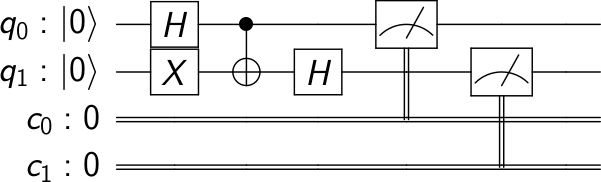
\includegraphics[scale=\myscale,scale=0.4]{figures/fig-circuit-latex}
\end{center}

\end{itemize}  

%--------------------------------------------------------------------
\subsection{Résultats}


Vérifier que le qubit de sortie attendu (avant mesure) est :
$$\ket\psi = \frac12\ket{0.0}-\frac12\ket{0.1}+\frac12\ket{1.0}+\frac12\ket{1.1}.$$

$$
\begin{array}{c}\ket0\\\otimes\\\ket0\end{array}  
\raise4ex\hbox{
\Qcircuit @C=1em @R=1.5em {
 & \gate{H} & \ctrl{1}  & \qw & \qwa \\
 & \gate{X} & \targ    & \gate{H} & \qwa \\
}
}
\qquad
\frac12\begin{array}{c}\ket0\\\otimes\\\ket0\end{array}
-\frac12\begin{array}{c}\ket0\\\otimes\\\ket1\end{array}
+ \frac12\begin{array}{c}\ket1\\\otimes\\\ket0\end{array}
+\frac12\begin{array}{c}\ket1\\\otimes\\\ket1\end{array}
$$

\medskip

Expérimentalement, voici un exemple de ce que renvoie le programme :
\mycenterline{\ci{'00': 245, '01': 240, '10': 273, '11': 242}}

L'affichage graphique met en évidence que chacune des $4$ mesures possibles
$0.0$, $0.1$, $1.0$, $1.1$ est équiprobable.

\begin{center}
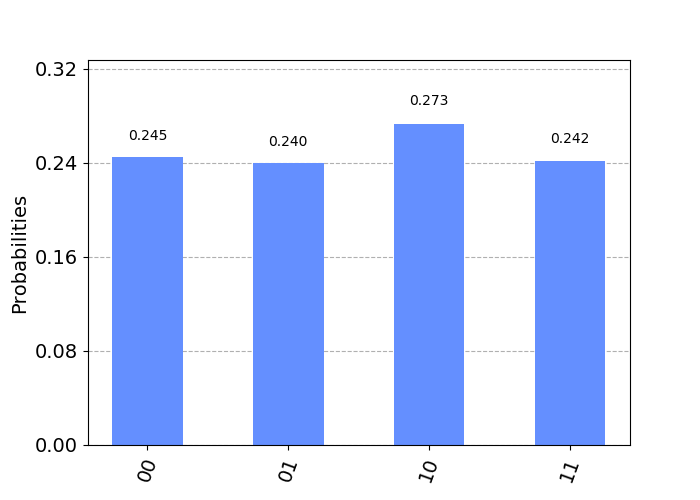
\includegraphics[scale=\myscale,scale=0.5]{figures/fig-qiskit-04}
\end{center}

\textbf{Piège !} Il y a une inversion entre notre notation \ket{0.1} (qui se mesure $0.1$) et celle de \qiskit{} \ci{'10'}. De même \ket{1.0} correspond à \ci{'01'}. En effet, \qiskit{} adopte la convention d'écriture des nombres binaires dans laquelle les bits sont écrits de droite à gauche.

$$
\begin{array}{cc}
\text{\'Ecriture d'un qubit} & \ket{c_0.c_1\ldots c_k} \\
\text{\'Ecriture de sa mesure} & c_0.c_1 \ldots c_k \\
\text{Notation \qiskit} & \text{\ci{'}}c_k \ \ldots\  c_1\ c_0\text{\ci{'}} \\
\end{array}
$$



\begin{exercicecours}
On souhaite vérifier expérimentalement que les deux circuits suivants sont équivalents (des entrées égales donnent des sorties égales).

{\large
$$
\raise3ex\hbox{\Qcircuit @C=1em @R=1em {
\lstick{\ket{\psi_1}} & \gate{H} & \ctrl{1} & \gate{H} & \qwa \\
\lstick{\ket{\psi_2}} & \gate{H} & \targ & \gate{H} & \qwa
}}\quad
\ket\psi
\qquad\qquad\qquad\qquad
\raise2ex\hbox{\Qcircuit @C=1em @R=1em {
\lstick{\ket{\psi_1}} & \targ &  \qw \\
\lstick{\ket{\psi_2}} & \ctrl{-1} &  \qw
}}\quad
\ket\psi
$$
}
Voici les étapes.
\begin{enumerate}
  \item Utiliser le moteur \ci{'statevector_simulator'}.
  \item Définir au hasard un qubit de norme $1$, $\ket{\psi_1}$. 
  Pour cela, on suit la méthode utilisée dans le programme de la section \ref{ssec:progstate} :
  \begin{itemize}
    \item définir des nombres complexes $\alpha_0$ et $\beta_0$ (choisis au hasard), 
    \item puis calculer la norme $n = \sqrt{|\alpha_0|^2+|\beta_0|^2}$, 
    \item puis $\alpha = \alpha_0/n$ et $\beta = \beta_0/n$ définissant $\ket{\psi_1}=\alpha\ket0+\beta\ket1$ de norme $1$,
    \item puis utiliser la fonction \ci{Initialize()} pour définir ce qubit.
  \end{itemize}
\item Définir de même $\ket{\psi_2}$.
  \item Définir le circuit \ci{circuit1} suivant le premier schéma et calculer le $2$-qubit $\ket\psi$ de sortie.
  \item Définir le circuit \ci{circuit2} suivant le second schéma et calculer le $2$-qubit $\ket{\psi'}$ de sortie.
  \item Comparer les sorties $\ket\psi$ et $\ket{\psi'}$.
\end{enumerate}
 On doit avoir $\ket\psi=\ket{\psi'}$ quel que soit le choix des entrées $\ket{\psi_1}$ et $\ket{\psi_2}$.

\end{exercicecours}

%--------------------------------------------------------------------
\subsection{Plus de qubits}

On peut bien sûr avoir davantage de qubits en entrée.
Voici un exemple de circuit avec trois qubits.
{\large
$$
\Qcircuit @C=1em @R=1em {
\lstick{\ket0} & \gate{H} & \ctrl{1} & \qw      & \qw      & \meter & \qwa \\
\lstick{\ket0} & \qw      & \targ    & \gate{H} & \ctrl{1} & \meter & \qwa \\
\lstick{\ket0} & \gate{H} & \qw      & \qw      & \targ    & \meter & \qwa \\
}
$$
}

\begin{lstlisting}
circuit = q.QuantumCircuit(3, 3)
circuit.h(0)      # Porte de Hadamard
circuit.h(2)      # Porte de Hadamard
circuit.cx(0, 1)  # CNOT
circuit.h(1)      # Porte de Hadamard
circuit.cx(1, 2)  # CNOT
circuit.measure([0,1,2], [0,1,2]) # Mesures
\end{lstlisting}

Voici un exemple de résultat :
\begin{center}
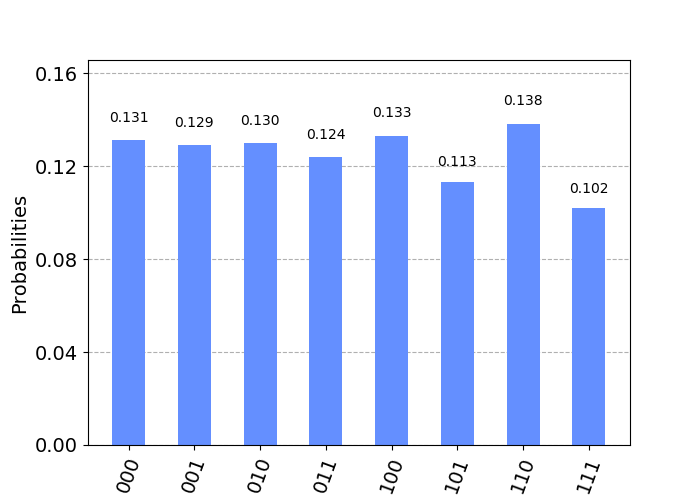
\includegraphics[scale=\myscale,scale=0.5]{figures/fig-qiskit-06}
\end{center}
%%%%%%%%%%%%%%%%%%%%%%%%%%%%%%%%%%%%%%%%%%%%%%%%%%%%%%%%%%%%%%%%%%%%%
\section{Utiliser un vrai ordinateur quantique}

%--------------------------------------------------------------------
\subsection{Accès à un ordinateur quantique}

Un des intérêts de \qiskit{} est que l'on peut exécuter ses programmes sur un ordinateur quantique !
En effet, IBM met à disposition du temps de calculs sur des véritables ordinateurs quantiques.
Cet accès est gratuit et ouvert à tous. Il faut cependant s'inscrire et patienter dans une file d'attente pour lancer son programme.

Voici les étapes préalables.
\begin{itemize}
  \item Se créer un compte sur le site \href{https://quantum-computing.ibm.com/}{\emph{quantum-computing.ibm.com}}.
  \item Récupérer son code d'accès (\emph{token}) qui est un un long mot de passe du genre \ci{'ce5a6210bb21...'}. Ce code n'est nécessaire que pour la première connexion.
\end{itemize}

%--------------------------------------------------------------------
\subsection{Programme}

Voici un circuit.
{\large
$$
\Qcircuit @C=1em @R=1em {
\lstick{\ket0} & \gate{H} & \ctrl{1} & \meter & \qwa   \\
\lstick{\ket0} & \qw      & \targ    & \meter & \qwa \\
}$$
}

Et voici le programme qui s'exécute à distance sur un vrai ordinateur quantique.
\begin{lstlisting}
import qiskit as q
from qiskit.tools.monitor import job_monitor
import matplotlib.pyplot as plt

### Partie A. Préparation

# Code à donner une fois seulement, ensuite commenter la ligne
q.IBMQ.save_account('ce5a6210bb21...')

q.IBMQ.load_account()

provider = q.IBMQ.get_provider(group='open')

print(provider.backends())  # Affiche les ordinateurs disponibles

backend = provider.get_backend('ibmq_essex')  # Choix d'un ordi disponible

### Partie B. Construction du circuit

circuit = q.QuantumCircuit(2, 2)
circuit.h(0)
circuit.cx(0, 1)
circuit.measure([0,1], [0,1])

### Partie C. Exécution 

job_exp = q.execute(circuit, backend=backend, shots=1000)
job_monitor(job_exp)

# Partie D. Résultats et visualisation

result_exp = job_exp.result()
counts_exp = result_exp.get_counts(circuit)
print(counts_exp)

q.visualization.plot_histogram(counts_exp)
plt.show()
\end{lstlisting}


%--------------------------------------------------------------------
\subsection{Explications}

\textbf{Partie A. Préparation.} La préparation consiste à donner son code d'accès (une seule fois), à choisir un accès libre (groupe \ci{'open'}), puis à choisir un ordinateur quantique parmi une liste disponible (ici \ci{'ibmq_essex'}).

\textbf{Partie B. Construction du circuit.} Comme d'habitude !

\textbf{Partie C. Exécution.} Presque comme d'habitude sauf qu'il faut être un peu plus patient pour disposer de l'accès et attendre la fin des calculs.

Voici la liste des messages qui informent l'utilisateur de l'avancement du travail :
\begin{lstlisting}
Job Status: job is being validated
Job Status: job is queued
Job Status: job is actively running
Job Status: job has successfully run
\end{lstlisting}

Si l'attente semble trop longue il existe un moyen de retrouver les résultats plus tard (à l'aide de la commande \ci{retrieve_job}).

%--------------------------------------------------------------------
\subsection{Résultats}

Voici un exemple de résultats sous forme numérique :
\mycenterline{\ci{'00': 449, '01': 60, '10': 28, '11': 463}}
et sous forme graphique :
\begin{center}
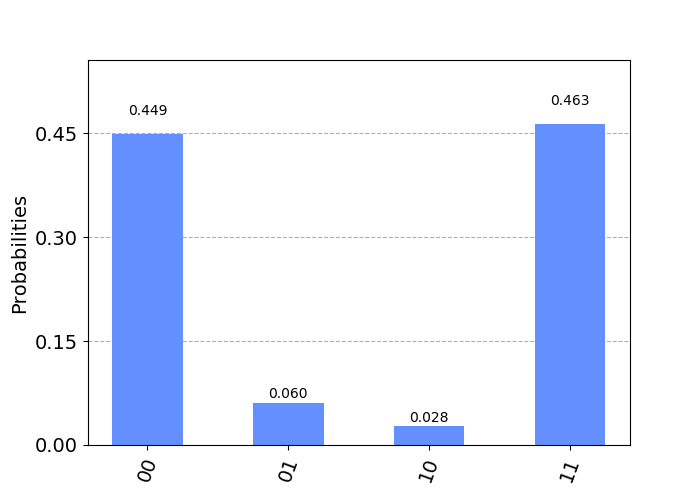
\includegraphics[scale=\myscale,scale=0.5]{figures/fig-qiskit-real}
\end{center}

Noter que l'état quantique de sortie (avant mesure) est
$\ket{\Phi^+} =  \frac1{\sqrt2} \ket{0.0} + \frac1{\sqrt2} \ket{1.1}$.
Les résultats devraient donc être uniquement mesurés en $0.0$ ou $1.1$ (avec des probabilités proches de $1/2$). Mais sur un véritable ordinateur quantique il y a des erreurs, qui ici produisent certaines mesures impossibles en théorie (ici $0.1$ et $1.0$).

On distingue deux causes qui font que l'on n'obtient pas exactement moitié/moitié pour les mesures $0.0$ et $1.1$ :
\begin{itemize}
  \item une cause probabiliste : il peut y avoir un écart entre les mesures et les probabilités théoriques attendues, écart dû au caractère aléatoire d'une mesure (comme le lancer d'une pièce de monnaie). Avec un grand nombre de lancers, cet écart diminue.
  \item une cause d'erreur physique : un ordinateur quantique n'est pas parfait, il peut y avoir des erreurs.
\end{itemize} 



%%%%%%%%%%%%%%%%%%%%%%%%%%%%%%%%%%%%%%%%%%%%%%%%%%%%%%%%%%%%%%%%%%%%%
\section{Codage super-dense}

\index{codage super-dense}

%--------------------------------------------------------------------
\subsection{Circuit}

Il s'agit de transmettre une information classique composée de deux bits $0.0$ ou $0.1$ ou $1.0$ ou $1.1$ en transmettant un seul qubit. 
On renvoie à la fin du chapitre \og{}Découverte de l'informatique quantique\fg{} pour les explications.
On rappelle le circuit en jeu :
$$
\Qcircuit @C=1em @R=1em {
\lstick{q_0=\ket0} & \gate{H} & \ctrl{1} & \gate{I,Z,X,XZ} & \ctrl{1} & \gate{H} & \meter       & \qw    & \qw \\
\lstick{q_1=\ket0} & \qw      & \targ    & \qw      & \targ    & \qw      & \qw          & \meter & \qw \\
\lstick{c_0=0}     & \qw      & \qw      & \qw      & \qw      & \qw      & \qw \qwx[-2] & \qw    & \qwa \\ 
\lstick{c_1=0}     & \qw      & \qw      & \qw      & \qw      & \qw      & \qw          & \qw \qwx[-2]   & \qwa \\
}$$

%--------------------------------------------------------------------
\subsection{Programme}

\begin{lstlisting}
import qiskit as q

### Partie A. Préparation
simulator = q.Aer.get_backend('qasm_simulator')

### Partie B. Construction du circuit

circuit = q.QuantumCircuit(2, 2)

## B.1 Préparation de l'état de Bell
circuit.h(0)  # Porte de Hadamard
circuit.cx(0, 1) # CNOT

message_alice = '01'  # choix entre '00', '01', '10', '11'

## B.2 Porte d'Alice selon message à transmettre
if message_alice == '00':
	circuit.iden(0)  # identité
elif message_alice == '01':
	circuit.z(0)     # porte Z
elif message_alice == '10':
	circuit.x(0)     # porte X
elif message_alice == '11':
	circuit.x(0)     # porte X
	circuit.z(0)     # suivi de porte Z	


## B.3 Décodage
circuit.cx(0, 1) # CNOT
circuit.h(0)  # Porte de Hadamard

## B.4 Mesures
circuit.measure([0,1], [0,1]) # Mesures

print(circuit.draw(output='text'))

### Partie C. Exécution 

# Lancer de 1000 simulations
job = q.execute(circuit, simulator, shots=1000)

# Partie D. Résultats

result = job.result()

# Comptage
counts = result.get_counts(circuit)
print("Nombre de '00', '01', '10' '11':",counts)
\end{lstlisting}


%--------------------------------------------------------------------
\subsection{Résultats}

Le programme s'utilise en choisissant le message qu'Alice envoie à Bob, par exemple \ci{
message_alice = '01'}. Dans ce cas, Alice ajoute une porte \mygate{Z} au circuit. La sortie mesurée est alors \ci{'01'} (dans $100\%$ des simulations). Testez les autres messages !

On rappelle la subtilité : si la mesure du qubit $q_0$ est $1$ et celle du qubit $q_1$ est $0$ alors on note globalement la mesure $1.0$ (correspondant à l'état quantique $\ket{1.0}$) mais \qiskit{} écrit cette même mesure \ci{'01'} (de la droite vers la gauche). Faites un choix pour votre programme et tenez-vous-y !

\end{document}
